\documentclass[11pt, a4paper, norsk]{NTNUoving}
\usepackage[utf8]{inputenc}
\usepackage[T1]{fontenc}
\usepackage{mathrsfs}
\newcommand{\RomanNumeralCaps}[1]
{\MakeUppercase{\romannumeral #1}}


\ovingnr{3}    % Nummer på innlevering
\semester{Haust 2022}
\fag{TMA4120}
\institutt{Institutt for matematiske fag}

\begin{document}
\section*{11.1}
\begin{oppgave}[2]
  Finner fundamental periode til oppgitte funksjoner.
  \begin{align*}
    \cos nx &: p = \frac{2\pi}{n} \\
    \sin nx &: p = \frac{2\pi}{n} \\
    \cos\frac{2\pi x}{k} &: p = k \\
    \sin\frac{2\pi x}{k} &: p = k \\
    \cos\frac{2\pi nx}{k} &: p = \frac{k}{n} \\
    \sin\frac{2\pi nx}{k} &: p = \frac{k}{n} \\
  \end{align*}
\end{oppgave}
\begin{oppgave}[15]
  Ser at funksjonen er hverken like eller odde i det gitte intervallet, så vi kan ikke bruke symmetriargument til å finne Fourierkoeffisienter.
  \begin{align*}
    a_{0}&=\frac{1}{2\pi}\int_{0}^{2\pi}x^{2}dx = \frac{4\pi^{2}}{3} \\
    a_{n}&=\frac{1}{\pi}\int_{0}^{2\pi}x^{2}\cos(nx)dx = \frac{8\pi^{2}}{3} \\
    a_{0}&=\frac{1}{2\pi}\int_{0}^{2\pi}x^{2}dx = \frac{8\pi^{3}}{3} \\
  \end{align*}
\end{oppgave}
\begin{oppgave}[17]
  Vi har en like funksjon, så $b_{n}=0$. Regner ut koeffisientene.
  \begin{align*}
    a_{0}&=\frac{1}{2\pi}\int_{-\pi}^{\pi}f(x)dx = \frac{1}{\pi}\int_{0}^{\pi}(\pi-x)dx = \frac{\pi}{2} \\
    a_{n}&=\frac{1}{\pi}\int_{-\pi}^{\pi}f(x)\cos(nx)dx = \frac{2}{\pi}\int_{0}^{\pi}(\pi-x)\cos(nx) dx = \frac{2-2\cos(\pi n)}{\pi n^{2}} = \frac{2-2(-1)^{n}}{\pi n^{2}}
  \end{align*}
  Bruker disse koeffisientene til å tegne $f(x)$ for $n=1$, $n=5$ og $n=50$: \\
  \[
    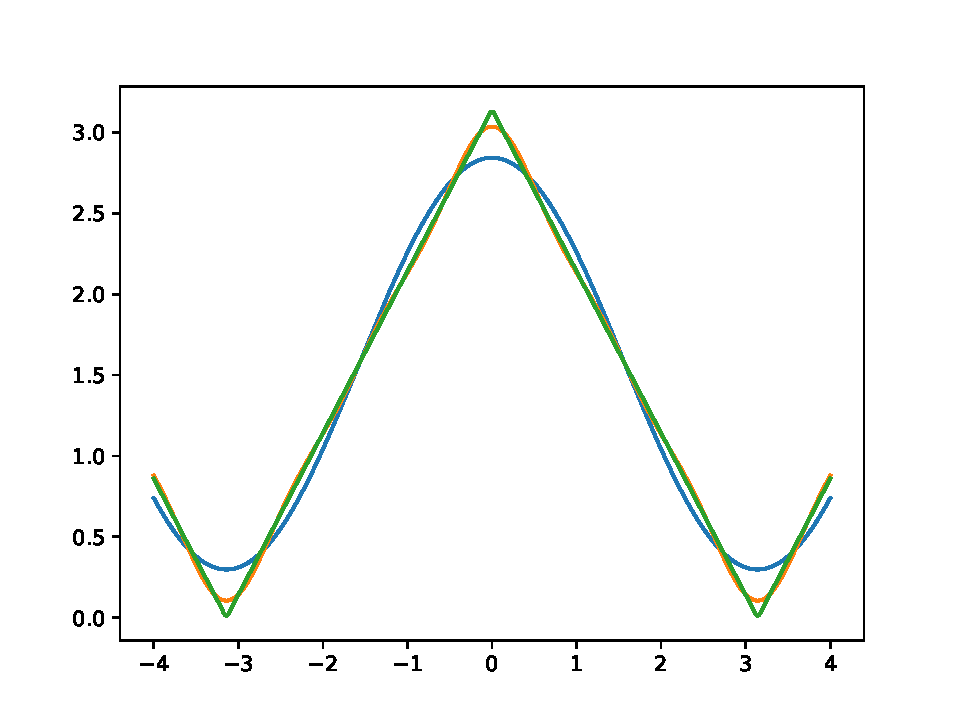
\includegraphics[scale=0.7]{11.1.17.pdf}
  \]
\end{oppgave}
\begin{oppgave}[21]
  Vi har en odde funksjon, så $a_{n}=0$. Regner ut koeffisientene.
  \begin{align*}
    b_{n}&=\frac{1}{\pi}\int_{-\pi}^{\pi}f(x)\sin(nx)dx = \frac{2}{\pi}\int_{0}^{\pi}(\pi-x)\sin(nx) dx = \frac{2\pi n-2\sin(\pi n)}{\pi n^{2}}
  \end{align*}
  Bruker disse koeffisientene til å tegne $f(x)$ for $n=1$, $n=5$ og $n=50$: \\
  \[
    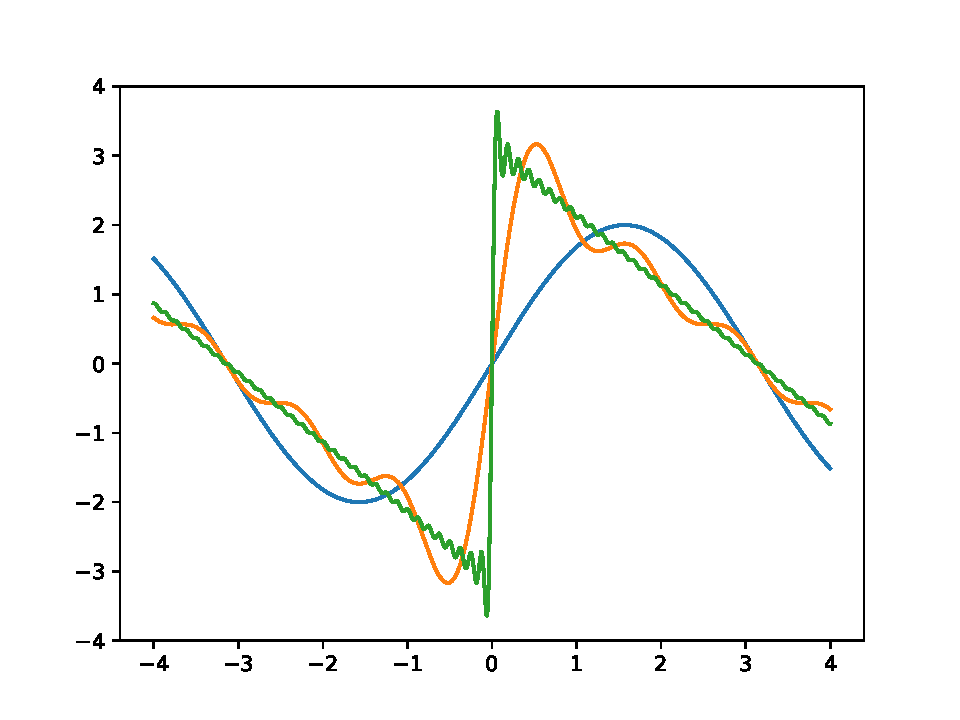
\includegraphics[scale=0.7]{11.1.19.pdf}
  \]
\end{oppgave}
\section*{11.2}
\begin{oppgave}[1]
\begin{align*}
  \text{Odde} &: x^{3}\cos(nx), x^{2}\tan(\pi x) \\
  \text{Like} &: e^{-|x|} \\
  \text{Hverken} &: e^{x}, \sinh(x)-\cosh(x)
\end{align*}
\end{oppgave}
\begin{oppgave}[10]
  Dette ligner veldig på oppgave 21. Gjør akkurat det samme, men med litt annen periode $L=4$.
  \begin{align*}
    b_{n}&=\frac{1}{4}\int_{-4}^{4}f(x)\sin\frac{n\pi x}{4}dx = \frac{1}{2}\int_{0}^{4}(4-x)\sin\frac{n\pi x}{4} dx = \frac{8\pi n-8\sin(\pi n)}{\pi^{2} n^{2}}
  \end{align*}
  Dette ser vi stemmer ved å plotte summen i python.
  \[
    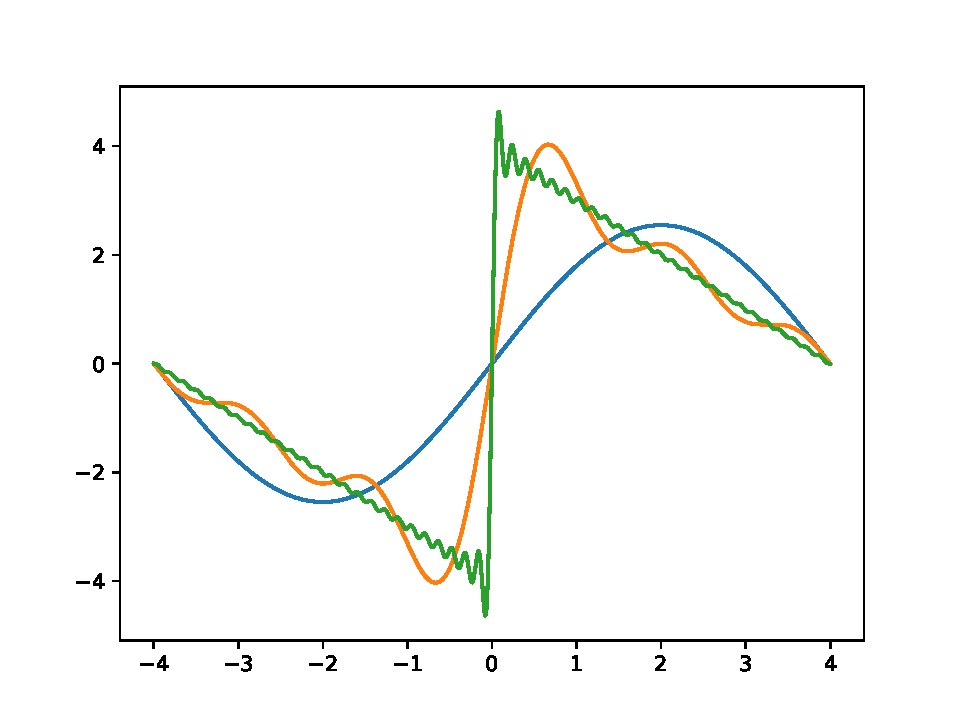
\includegraphics[scale=0.7]{11.2.10.pdf}
  \]
\end{oppgave}
\begin{oppgave}[17]
  Igjen har vi en funksjon som ligner veldig på en tidligere oppgave. Her har vi periode $L=1$. Koeffisientene blir
  \begin{align*}
    a_{0}&=\frac{1}{2}\int_{-1}^{1}f(x)dx = \int_{0}^{1}(1-x)dx = \frac{1}{2} \\
    a_{n}&=\int_{-1}^{1}f(x)\cos(n\pi x)dx = 2\int_{0}^{1}(1-x)\cos(n\pi x) dx = \frac{2-2\cos(\pi n)}{\pi^{2} n^{2}} = \frac{2-2(-1)^{n}}{\pi^{2} n^{2}}
  \end{align*}
  Plotter summen og får
  \[
    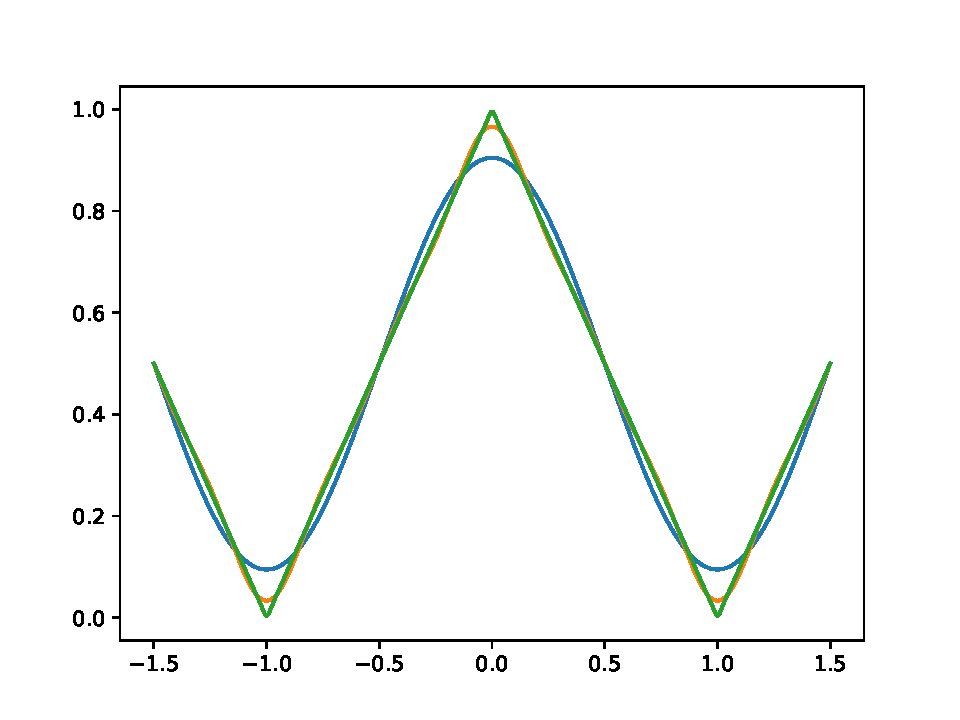
\includegraphics[scale=0.7]{11.2.17.pdf}
  \]
\end{oppgave}
\begin{oppgave}[24]
  Deler oppgaven inn i a) og b), som henholdsvis svarer til Fourier cosinus- og sinusrekken til funksjonen.
  \begin{punkt}
    Funksjonen er like og har periode med $L=4$. Ser at den har midtpunkt i $y=1/2\Rightarrow a_{0}=1/2$. Regner så ut koeffisientene.
    \begin{align*}
      a_{n}=\frac{1}{2}\int_{2}^{4}\cos\frac{n\pi x}{4}dx = \frac{2(\sin(\pi n)-\sin\frac{\pi n}{2})}{\pi n} = -\frac{2}{\pi n}\sin\frac{n\pi}{2}
    \end{align*}
  \end{punkt}
  \begin{punkt}
    Denne funksjonen blir odde, men har fortsatt periode med $L = 4$. Koeffisientene blir
    \begin{align*}
      b_{n}=\frac{1}{2}\int_{2}^{4}\sin\frac{n\pi x}{4} dx= \frac{2(\cos\frac{\pi n}{2}-\cos(\pi n))}{\pi n} = \frac{2}{\pi n}\left(\cos\frac{n\pi}{2}-(1)^{n}\right)
    \end{align*}
  \end{punkt}
  Under er Fourier cosinus- og sinusrekken skissert i python.
  \begin{center}
    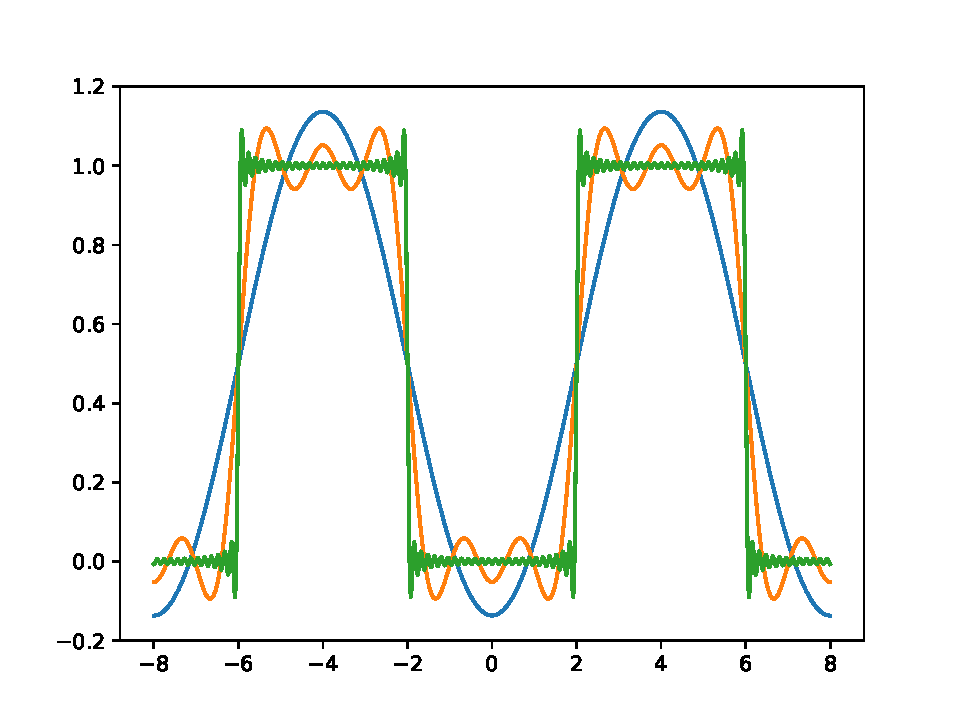
\includegraphics[scale=0.42]{11.2.24}
    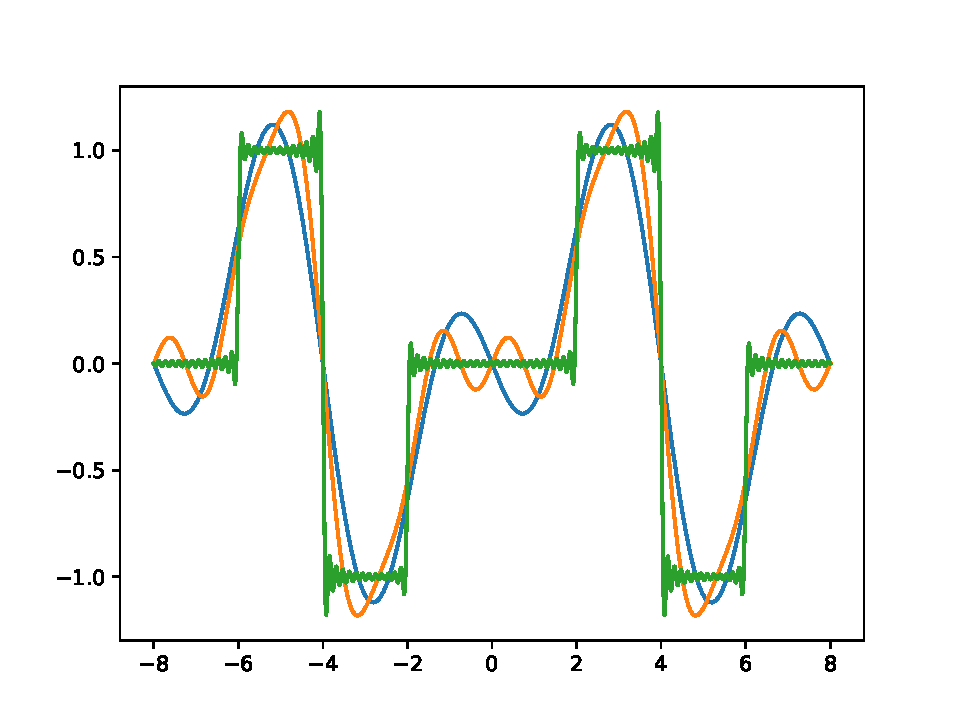
\includegraphics[scale=0.42]{11.2.24b}
  \end{center}
\end{oppgave}
\newpage
\begin{oppgave}[29]
  Ser ganske greit at Fourier sinusrekken i dette tilfellet gir $\sin(x)$. Fourier cosinusrekken, derimot, krever litt regning. Vi har en like funksjon med periode $p=2\pi$.
  \begin{align*}
    a_{0}&= \frac{1}{\pi}\int_{0}^{\pi}\sin(x)dx = \frac{2}{\pi} \\
    a_{n}&=\frac{2}{\pi}\int_{0}^{\pi}\sin(x)\cos(n x)dx = \frac{2(\cos(\pi n)+1)}{\pi - \pi n^{2}}
    = \frac{2(1+(-1)^{n})}{\pi - \pi n^{2}}
  \end{align*}
  Plotter i python for å sjekke at det er riktig.
  \[
    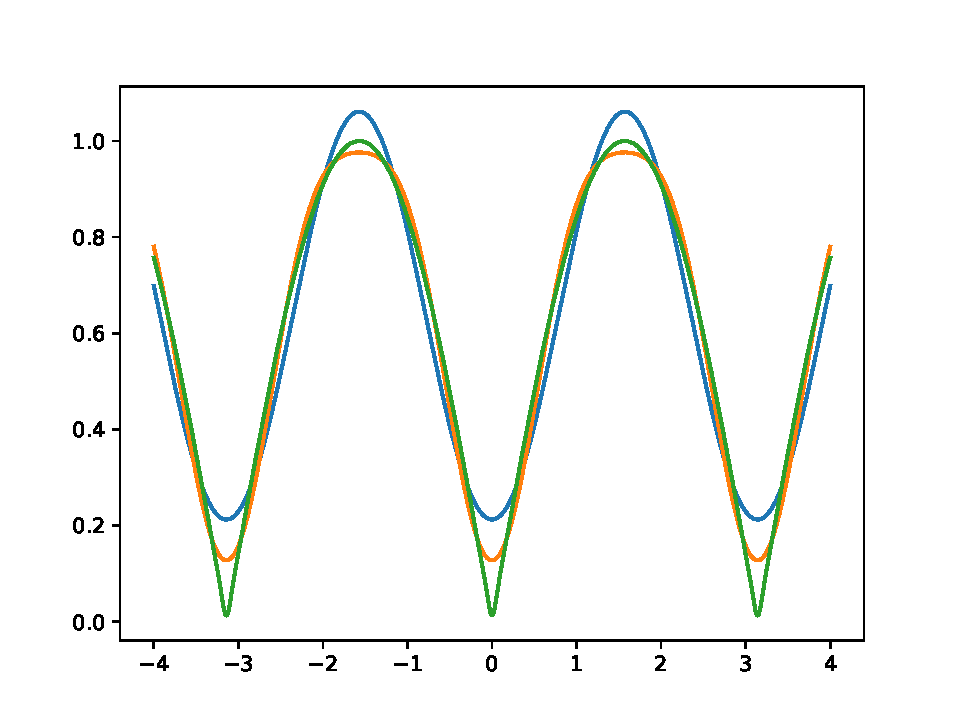
\includegraphics[scale=0.7]{11.2.29.pdf}
  \]
\end{oppgave}
\section*{11.3}
\begin{oppgave}[15]
  Begynner med å finne Fourierrekken til $r(t)$. Observerer at $r(t)$ er odde, slik at $a_{n}=0$. Får da
  \begin{align*}
    b_{n}=\frac{2}{\pi}\int_{0}^{\pi}t(\pi^{2}-t^{2})\sin(n t) dt = -\frac{12(-1)^{n}}{n^{3}}
  \end{align*}
  Det betyr at
  \[
    r(t) = 12\sin(t) - \frac{12}{2^{3}}\sin(2t) + \frac{12}{3^{3}}\sin(3t) - ...
  \]
  Har da
  \[
    y''+c y' + y = -\frac{12(-1)^{n}}{n^{3}}\sin(nt)
  \]
  med
  \[
    y_{n} = A_{n}\cos(nt)+B_{n}\sin(nt)
  \]
\end{oppgave}
\end{document}
